\documentclass[a4paper]{report}

%====================== PACKAGES ======================

\usepackage[french]{babel}
\usepackage[utf8x]{inputenc}

%pour gérer les positionnement d'images
\usepackage{float}
\usepackage{amsmath}
\usepackage{graphicx}
\usepackage[colorinlistoftodos]{todonotes}
\usepackage{url}
%pour les informations sur un document compilé en PDF et les liens externes / internes
\usepackage{hyperref}
%pour la mise en page des tableaux
\usepackage{array}
\usepackage{tabularx}
%pour utiliser \floatbarrier
%\usepackage{placeins}
%\usepackage{floatrow}
%espacement entre les lignes
\usepackage{setspace}
%modifier la mise en page de l'abstract
\usepackage{abstract}
%police et mise en page (marges) du document
\usepackage[T1]{fontenc}
\usepackage[top=2cm, bottom=2cm, left=2cm, right=2cm]{geometry}
%Pour les galerie d'images
\usepackage{subfig}

%====================== INFORMATION ET REGLES ======================

%rajouter les numérotation pour les \paragraphe et \subparagraphe
\setcounter{secnumdepth}{4}
\setcounter{tocdepth}{4}

\hypersetup{                            % Information sur le document
pdfauthor = {IBRIR Yassine,
            MARTINS MOSCA Jerôme,
            RAHIER Valentine,
            VIOLETTE Paulin},          % Auteurs
pdftitle = {L.I.D.E. -
            Application web pour le developpement},           % Titre du document
pdfsubject = {Rapport de Projet},       % Sujet
pdfkeywords = {},  % Mots-clefs
pdfstartview={FitH}}                    % ajuste la page à la largueur de l'écran
%pdfcreator = {MikTeX},% Logiciel qui a crée le document
%pdfproducer = {}} % Société avec produit le logiciel

%======================== DEBUT DU DOCUMENT ========================

\begin{document}

%régler l'espacement entre les lignes
\newcommand{\HRule}{\rule{\linewidth}{0.5mm}}

%page de garde
\begin{titlepage}
\begin{center}

% Upper part of the page. The '~' is needed because only works if a paragraph has started.

\includegraphics[width=0.35\textwidth]{./img/logo}~\\[1cm]

\textsc{\LARGE M1 Informatique}\\[1.5cm]

\textsc{\Large Concrétisation Disciplinaire}\\[0.5cm]

% Title
\HRule \\[0.4cm]

{\huge \bfseries L.I.D.E.\\
Application Web de Développement \\[0.4cm] }

\HRule \\[1.5cm]

% Author and supervisor
\begin{minipage}{0.4\textwidth}
\begin{flushleft} \large
\emph{Auteurs}\\
Yassine \textsc{Ibrir}\\
Jerôme \textsc{Martins Mosca}\\
Valentine \textsc{Rahier}\\
Paulin \textsc{Violette}\\
\end{flushleft}
\end{minipage}
\begin{minipage}{0.4\textwidth}
\begin{flushright} \large
\emph{Chefs de projet}\\
Alice \textsc{Bazanté}\\
Sullivan \textsc{Chevallier}\\
Pierre-Olivier \textsc{Mainfroid}\\
\emph{Référent:} \\
Laurent \textsc{Garcia}
\end{flushright}
\end{minipage}

\vfill

% Bottom of the page
{\large Octobre - Décembre 2017}

\end{center}
\end{titlepage}


%page blanche
\newpage
~
%ne pas numéroter cette page
\thispagestyle{empty}
\newpage

\renewcommand{\abstractnamefont}{\normalfont\Large\bfseries}
%\renewcommand{\abstracttextfont}{\normalfont\Huge}

\begin{abstract}
\hskip7mm

\begin{spacing}{1.3}

%Résumé

Lorem ipsum dolor sit amet, consectetur adipiscing elit. Sed non risus. Suspendisse lectus tortor, dignissim sit amet, adipiscing nec, ultricies sed, dolor. Cras elementum ultrices diam. Maecenas ligula massa, varius a, semper congue, euismod non, mi. Proin porttitor, orci nec nonummy molestie, enim est eleifend mi, non fermentum diam nisl sit amet erat. Duis semper. Duis arcu massa, scelerisque vitae, consequat in, pretium a, enim. Pellentesque congue. Ut in risus volutpat libero pharetra tempor. Cras vestibulum bibendum augue. Praesent egestas leo in pede. Praesent blandit odio eu enim. Pellentesque sed dui ut augue blandit sodales. Vestibulum ante ipsum primis in faucibus orci luctus et ultrices posuere cubilia Curae; Aliquam nibh. Mauris ac mauris sed pede pellentesque fermentum. Maecenas adipiscing ante non diam sodales hendrerit. Ut velit mauris, egestas sed, gravida nec, ornare ut, mi. Aenean ut orci vel massa suscipit pulvinar. Nulla sollicitudin. Fusce varius, ligula non tempus aliquam, nunc turpis ullamcorper nibh, in tempus sapien eros vitae ligula. Pellentesque rhoncus nunc et augue. Integer id felis. Curabitur aliquet pellentesque diam. Integer quis metus vitae elit lobortis egestas. Lorem ipsum dolor sit amet, consectetuer adipiscing elit. Morbi vel erat non mauris convallis vehicula. Nulla et sapien. Integer tortor tellus, aliquam faucibus, convallis id, congue eu, quam. Mauris ullamcorper felis vitae erat. Proin feugiat, augue non elementum posuere, metus purus iaculis lectus, et tristique ligula justo vitae magna. Aliquam convallis sollicitudin purus. Praesent aliquam, enim at fermentum mollis, ligula massa adipiscing nisl, ac euismod nibh nisl eu lectus. Fusce vulputate sem at sapien. Vivamus leo. Aliquam euismod libero eu enim. Nulla nec felis sed leo placerat imperdiet. Aenean suscipit nulla in justo. Suspendisse cursus rutrum augue. Nulla tincidunt tincidunt mi. Curabitur iaculis, lorem vel rhoncus faucibus, felis magna fermentum augue, et ultricies lacus lorem varius purus. Curabitur eu amet.

\end{spacing}
\end{abstract}

\tableofcontents
\thispagestyle{empty}
\setcounter{page}{0}
%ne pas numéroter le sommaire

\newpage

%espacement entre les lignes d'un tableau
\renewcommand{\arraystretch}{1.5}

%====================== INCLUSION DES PARTIES ======================

~
\thispagestyle{empty}
%recommencer la numérotation des pages à "1"
\setcounter{page}{0}
\newpage

%Ici faire les inputs de toutes les parties

\chapter{Présentation du projet}

\par L'installation de compilateurs peut se montrer compliquée pour les étudiants novices qui suivent les cours d'initiation à la programmation. L'Université d'Angers a donc souhaité simplifier leur apprentissage en centralisant tous les besoins dans un outil de développement en ligne.

\section{Sujet}
%Présentation du sujet : entreprise, encadrement

\par Notre objectif était de réaliser la première version d'un environnement de développement simplifié accessible à partir d'un navigateur web. Il permet d'écrire et de compiler du code rapidement et simplement sans avoir à installer de compilateur sur le poste client (la compilation s'effectuant sur le serveur). Cet outil pourrait être utilisé, dans le cadre des enseignements à l'Université d'Angers, dans plusieurs unités dès la L1 jusqu'à la L3. \\

\par Certaines caractéristiques nous étaient demandées : 

\begin{itemize}

	\item l'édition de code dans un éditeur proposant la coloration syntaxique
	\item la possibilité de compiler le code depuis des compilateurs installés sur le serveur. Le logiciel devra prendre en compte différents langages afin d’être utilisable dans différentes UE
	\item l'accès aux messages d'erreur de la compilation
	\item l'exécution de l'application compilée sur le serveur avec affichage de la sortie
	\item des fonctionnalités avancées devaient être développées telles que l’intégration du débogueur, une gestion plus poussée de l’ensemble de fichiers composant un projet, l'auto-complétion du code, l'intégration d’outils d’analyse

\end{itemize}


\section{Problématique soulevée}

\par L'enjeu principal de ce projet était la sécurité du serveur. En effet, lorsqu'un étudiant tente d'exécuter un programme qui contient des erreurs ou qui demande trop de mémoire CPU, il ne faut pas que le serveur qui gère l'exécution ni les exécutions d'autres étudiants soient ralentis ou bloqués. Pour pallier ces problèmes, nous nous devions d'élaborer une architecture sécurisée afin d'éviter les failles.


\section{Choix des principaux outils et technologies}

\par Lors de la première séance de concrétisation disciplinaire, nos chefs de projet nous ont proposé d'utiliser le framework Symfony pour la réalisation de notre application. Ce framework force à organiser le code et permet une gestion simple de la base de données qui ne dépend pas du type de base de données. De plus, Symfony permet une génération simple des pages grâce à ses controllers et au moteur de template twig.\
Un autre avantage de Symfony est la possibilité d'utiliser des bundles (par exemple, FOSUserBundle permet la gestion des utilisateurs) qui simplifie et accélère véritablement la réalisation des projets. \\

\par Nous avons décidé de placer sous licence libre notre application, c'est pourquoi nous avons choisi MariaDB comme système de gestion de la base de données. De plus, MariaDB a l'avantage d'être légère. \\

\par L'interface graphique a été réalisé grâce au framework Bootstrap qui fournit un thème de base cohérent et esthétique. Bootstrap est simple à utiliser car il se base sur des classes CSS. \\

\par Le choix de la conteneurisation, et plus particulièrement Docker, s'est vite imposé dans l'architecture du serveur. Docker est une méthode de conteneurisation légère qui permet de travailler toujours sur le même environnement (la même image est réutilisée autant de fois que nécessaire) et qui nous a permis d'isoler les compilations et exécutions des programmes.

\section{Répartition des tâches}

\par Afin de travailler efficacement, nous avons séparé le projet en 4 parties autonomes plus ou moins autonomes: Paulin s'est occupé de l'interface graphique, Yassine de l'administration, Jérôme de l'architecture du serveur et Valentine de la communication entre les serveurs.

\subsection{Planning}

Faire le planning
%Paulin VIOLETTE
%Si t'as pas bossé sur l'interface utilisateur t'y touche pas.
%Sauf si la personne dont le nom est écris en haut te dis d'y toucher.
%Deso Paulin moi j'y ai touché
\chapter{Interface Utilisateur}

\section{Présentation}

%Mettre l'image de ma super interface grave stylé
\begin{figure}[h]
  \centering
  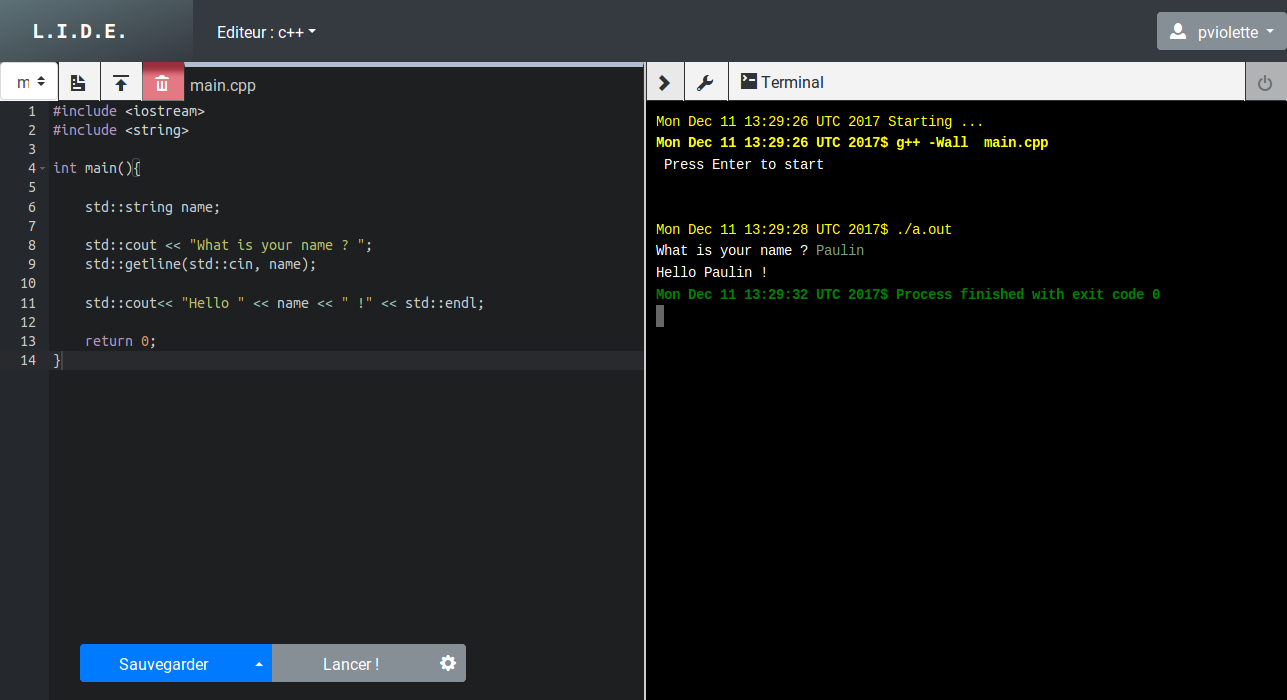
\includegraphics[width=0.8\textwidth]{./img/frontend/example1.png}
  \caption{Interface utilisateur en utilisation}
  \label{}
\end{figure}

Une fois l'utilisateur connecté, il est redirigé vers l'interface de l'application : un éditeur de texte et une console.
L'interface est divisée en quatre parties :
\begin{itemize}
  \item La barre de navigation, contenant les liens vers les autres parties du site (gestion de compte...)
  \item La barre d'outils, qui contient des contrôles spécifiques à l'application
  \item L'éditeur, implémenté par le plugin Ace
  \item La console, implémentée par le plugin jqconsole
\end{itemize}

\section{Outils utilisés}
%Editeur ace
%SweetAlert2 pour les alertes trop swag
%JQConsole vite zef parceque c'est valou qui l'a fait

En plus des outils déjà décrits dans la section \ref{sec-principaux-outils}, l'interface utilisateur utilise plusieurs plugins Javascript.

L'éditeur de texte est Ace\footnote{Voir \url{https://ace.c9.io/}}, un éditeur de texte pour le web supportant la coloration syntaxique de près de 110 langages, mis à disposition sous licence BSD et maintenu comme le principal éditeur pour l'IDE AWS Cloud9. Cet éditeur a pour avantage de supporter de nombreuses fonctionnalités, parmi lesquelles :
\

\begin{itemize}
  \item L'indentation automatique
  \item Chercher/Remplacer avec des expressions régulières
  \item Changement entre tabulation avec des espaces ("soft tab") ou avec une réelle tabulation (caractère \\t, "hard tab").
  \item Numérotage des lignes
  \item Et bien d'autres...
\end{itemize}

Toutes ces raisons nous ont poussés à utiliser ce plugin.

Afin de gérer la console, nous avons choisi d'utiliser le plugin jqconsole (Plus de détails en \ref{subsec-terminal}).

Dernièrement, pour afficher les alertes relatives à l'interface, nous utilisons le plugin SweetAlert2\footnote{Voir \url{https://limonte.github.io/sweetalert2/}} qui nous permet d'avoir des alertes personnalisables et bien plus esthétiques que les alertes classiques.

\subsection{Organisation des templates TWIG}

Le template twig de l'application, \texttt{index.html.twig}, hérite du template \texttt{layout.html.twig}, qui défini une base pour l'application, et qui contient la barre de navigation. Nous avons également créer differents templates pour les modales d'options (de personnalisation, de lancement, d'importation et de création de fichier).

Les templates du bundle FOS (gérant la partie utilisateur du site) sont également redéfini pour s'integrer avec le reste de l'application.

\section{Environnement de Développement}

\subsection{Gestions des langages}
Blabla DB changement de langage

\subsection{Personnalisation}

Toute personne ayant déjà travaillé en groupe sur un projet informatique a pu remarquer que chacun à ses préférences de thème pour un éditeur : certains préfèrent un fond sombre, d'autres un fond clair, etc... L'éditeur Ace est facilement personnalisable et dispose, par défaut, de 24 thèmes. Il était donc assez rapide d'implémenter un formulaire permettant à l'utilisateur de choisir le thème qui lui convient le mieux, lui permettant ainsi de facilement s'approprier son outil de travail.

La police est également personnalisable, permettant à chacun d'utiliser une taille de police qui lui convient.

La console ayant un style implémenté par CSS, il fut de même aisé de créer des thèmes qui s'appliquent grâce à une classe attribuée à l'élément div contenant la console. Pour l'instant, seuls trois styles de console sont implémentés, mais il serait aisé d'en ajouter d'autres dans des versions futures. Chaque style a une classe maîtresse \emph{.console-nom\_style}. On redéfinit ensuite les classes \emph{jqconsole} grâce aux sélecteurs CSS (voir le fichier \emph{console.css}).

Tous ces changements sont pour l'instant uniquement gérés en local (voir fichier \emph{options.js}).

\begin{figure}[!h]
\centering
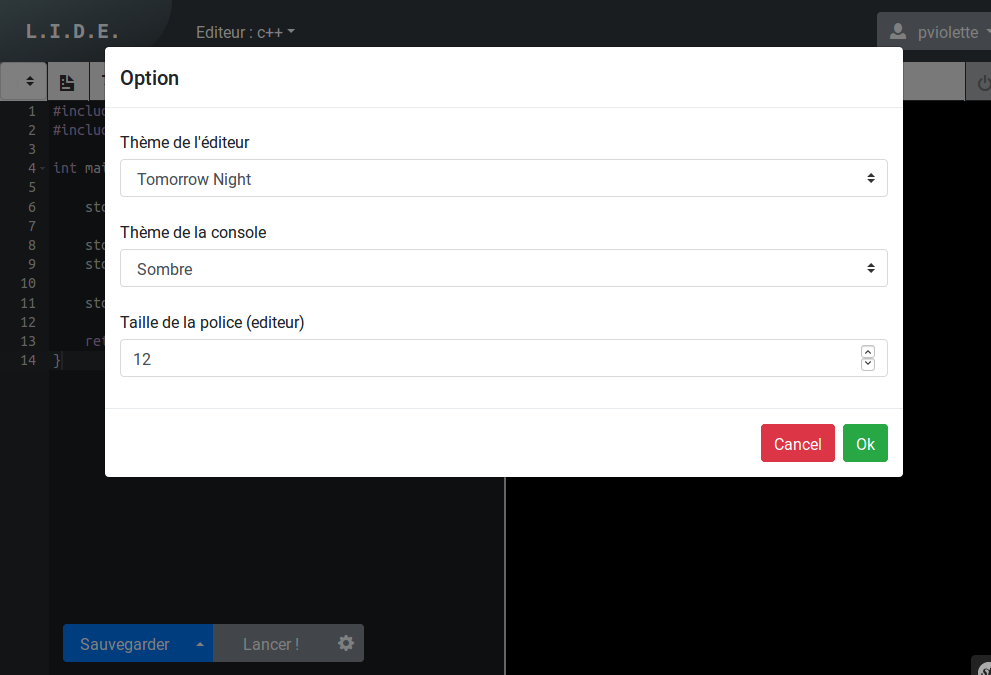
\includegraphics[width=0.8\textwidth]{./img/frontend/example_personnalisation.png}
\caption{Formulaire permettant la personnalisation de l'interface}
\end{figure}

\subsection{Gestions des fichiers}
Tel un véritable EDI, notre application permet la gestion de multiples fichiers. Cette gestion est effectuée sur le navigateur par du javascript.

Les fichiers sont enregistrés dans un prototype contenant deux champs : \emph{name}, le nom du fichier, et \emph{content} son contenu. Ces prototypes sont ensuite stockés dans la variable globale \emph{files}, un tableau de fichier. À chaque changement de fichier en cours d'édition, le contenu de l'éditeur est sauvegardé et est ensuite remplacé par le contenu du nouveau fichier à éditer.

Les fichiers peuvent être créer de deux façons : soit en important un fichier depuis son ordinateur (bouton importation), soit par création à partir de modèles définis par l'administrateur pour le langage.
On laisse également la possibilité de créer des fichiers vides (par exemple pour créer un fichier de données utilisé lors de l'exécution du programme).


\section{Compilation et exécution}

\subsection{Formulaire}

Le formulaire pour compiler et exécuter est généré par Symfony à partir de l'entity \texttt{Execution} et de la classe \texttt{ExecutionType}. Le formulaire comporte 7 champs :
\begin{itemize}
  \item Les paramètres de compilations : arguments passés au compilateurs
  \item Les paramètres de lancement : arguments donnés au programme
  \item Fichiers additionnels : l'utilisateur peut choisir des fichiers depuis son ordinateurs qui seront joints aux fichiers présents dans l'IDE
  \item Une option Compilation Uniquement : si activée, seule la compilation sera effectuée; le programme ne sera pas lancé
  \item{ Un choix de gestion du flux d'entrée :
  \begin{itemize}
    \item Aucun : aucune gestion des entrées n'est effectuée
    \item Interactive : entrée interactive, l'utilisateur écrit sur le flux d'entrée au fur et à mesure de l'exécution du programme.
    \item Texte : les entrées sont définie à l'avance, le programme utilise un fichier comme flux d'entrée.
  \end{itemize}}
  \item Les entrées à donner au programme : seulement si le mode de gestion des entrées Texte est sélectionné.
  \item Un champs caché alimenté par le javascript, contenant le JSON correspondant à la liste des fichiers.
\end{itemize}

\subsection{Lancement de la compilation et de l'exécution}

Le lancement de la compilation et de l'exécution du code écrit est lancé par l'appui sur le bouton "Lancer" qui appelle une fonction JS envoyant une requête AJAX vers la méthode \texttt{ConsoleController::execAction} (fichier ConsoleController.php). Cette requête contient le formulaire qui est ensuite traité : les fichiers vont être écrits dans le système du fichier dans un dossier temporaire, le script de lancement et d'exécution correspondant au langage est récupéré dans la base de données et placé dans ce même répertoire. Une commande, qui va permettre de lancer le docker, est ensuite construite. Cette commande va :
\begin{itemize}
  \item Stopper le container de l'utilisateur s'il existe.
  \item{Lancer un container basé sur l'image correspondante au langage, de nom \emph{id\_[id\_user]A}, paramétré pour être supprimé à la fin de l'exécution de la commande de lancement. Cette commande de lancement va :
  \begin{itemize}
    \item Récupérer le script de lancement sur le serveur de l'application via un wget
    \item Attribuer les droits d'exécution sur ce script
    \item Une commande sed remplaçant les caractères indésirables (dus à la base de données).
    \item Lancer le script avec les bons paramètres
  \end{itemize}}
\end{itemize}

Les paramètres du script à lancer sont :
\begin{itemize}
  \item \texttt{-o 'options\_de\_compilation'}, pour les paramètres à passer au compilateur
  \item \texttt{-f 'fichier1 fichier2...'}, la liste des fichiers de l'utilisateur (récupérée par un wget)
  \item \texttt{-i fichier}, le nom du fichier contenant les inputs s'il est nécessaire
  \item \texttt{-n}, pour un mode non interactif.
  \item \texttt{-a 'agr0 arg1 ...'}, les arguments à donner au programme
  \item \texttt{-c}, pour uniquement effectuer la compilation
  \item \texttt{-w 'wget\_adr'} l'adresse où effectuer le wget.
\end{itemize}

\subsection{Terminal}
\label{subsec-terminal}

\par La mise en place de la console proposait deux options : soit la création d'une vue ad-hoc soit l'intégration d'une vue déjà existante.

\par Notre choix s'est vite tourné vers l'intégration d'une vue déjà existante. La création d'une vue nous aurait certes donné une modularité de la console en ce qui concerne les modifications mais, la console une fois implémentée n'a pas nécessairement besoin de modifications.

\par Après étude de rentabilité, nous avons décidé d'implémenter la vue JQConsole \footnote{https://github.com/replit/jq-console} (utilisée dans repl.it\footnote{\url{https://repl.it/}}, un projet similaire au nôtre) qui correspondait exactement à nos besoins. En plus d'être esthétique, son code source était placé sous licence libre et toutes les fonctions qui nous étaient nécessaires étaient déjà implémentées. L'inconvénient principal est que la modification du code source peut se montrer compliqué, celui-ci étant rédigé en CoffeeScript et étant assez compliqué.

\par Nous n'avions donc plus qu'à intégrer la vue JQConsole à notre interface et faire appel aux bonnes fonctions (notamment JQConsole.Write qui permet d'afficher du texte dans la console et JQConsole.Prompt qui permet de lire du texte) pour obtenir notre console.

\section{Problème rencontré et amélioration possible}

\subsection{Rendre l'interface Responsive}
Un des problèmes de l'interface actuelle est son manque d'adaptabilité sur les plus petits écrans, le design actuel n'ayant pas été conçu dans le but de répondre à cette problématique. Cela est principalement dû au manque d'expérience en web qui nous a mené vers quelque chose de fonctionnel sur ordinateur qui n'est l'est pas sur les plateformes mobiles aux écrans plus petits. C'est une amélioration qu'il serait souhaitable de réaliser dans un version future.

\subsection{Persistance des options de personnalisation et de compilation}

Actuellement, la persistance des options de compilation ou de personnalisation n'est pas assurée. Cette fonctionnalité n'a pas été implémentée principalement par manque de temps mais pourrait rapidement être implémentée en ajoutant les champs nécessaires dans la base de données, afin de lier les préférences à un utilisateur, et en implémentant une méthode renvoyant les choix effectués dans le formulaire de personnalisation au serveur via une requête AJAX, afin que ces choix soit sauvegardés en base de données.

\newpage

%récupérer les citation avec "/footnotemark"
\nocite{*}

%choix du style de la biblio
%\bibliographystyle{plain}
%inclusion de la biblio
%\bibliography{bibliographie.bib}
%voir wiki pour plus d'information sur la syntaxe des entrées d'une bibliographie

\end{document}